\documentclass[11pt, titlepage]{article}

%% Language and font encodings
\usepackage[english]{babel}
\usepackage[utf8x]{inputenc}
%% Sets page size and margins

%% Useful packages
\usepackage{amsmath}
\usepackage{siunitx}
\usepackage{graphicx}
\usepackage{xspace}
\usepackage{float}
\usepackage{authblk}
\usepackage{minted}
\usepackage{afterpage}
\usepackage[numbers]{natbib}
\usepackage[compatibility=false]{caption}
\usepackage[colorinlistoftodos]{todonotes}
\usepackage[colorlinks=true, allcolors=blue]{hyperref}
\usepackage[author={Giovanni Garufi}]{pdfcomment}
\graphicspath{ {images/} }

\title{Version Control Systems: Diffing with Structure
\\ Thesis}
\author{Giovanni Garufi\\5685109\\[1cm]{Supervisors: \\
    Wouter Swierstra \\
    Victor Cacciari Miraldo}}
\affil{Department of Computing Science\\University of Utrecht}

\newcommand{\toHaskell}[1]{\mintinline{haskell}{#1}\xspace}
\newcommand{\toClojure}[1]{\mintinline{clj}{#1}\xspace}
\newcommand{\diffthree}{\emph{diff3}}
\newcommand{\diff}{\emph{diff}}
\newcommand{\SOP}{SOP\xspace}
\newcommand{\alins}{\toHaskell{Alins}}
\newcommand{\aldel}{\toHaskell{Aldel}}
\newcommand{\alspn}{\toHaskell{Alspn}}
\newcommand{\almu}{\toHaskell{Almu}}
\newcommand{\scp}{\toHaskell{Scp}}
\newcommand{\scns}{\toHaskell{Scns}}
\newcommand{\schg}{\toHaskell{Schg}}
\newcommand{\ains}{\toHaskell{Ains}}
\newcommand{\adel}{\toHaskell{Adel}}
\newcommand{\amod}{\toHaskell{Amod}}
\newcommand{\azero}{\toHaskell{A0}}

\begin{document}  


\maketitle
\tableofcontents


\section{Introduction}
Version control systems (VCS) have been steadily becoming an ubiquitous and central 
tool in programming. Many big projects, with hundreds of collaborators, 
fundamentally rely on these kind of tools to enable different users to interact 
with one another and to keep a structured log of the units of change. 
At the heart of most modern VCS is the Unix \diff utility. This tool computes a 
line-by-line difference between two files of text, determining the smallest set 
of insertions or deletions of lines that transform one file into the other. This sequence of transformations produced by \diff is called an edit script. 
When two collaborators have modified the same source file in independent ways and the VCS wants to reconcile the two independent changes into a single one it will attempt to produce a single edit script that encompasses both changes, this is commonly referred to 
as a merge. This operation is clearly not always possible: if two collaborators have modified the same line the two resulting edit scripts will ``overlap'', it is not clear which one of the two modifications should be picked.  The algorithm used to calculate these merges in most VCS is \diff3, which works by calculating the two edit-scripts with \diff, and attempting to merge them.
\\
In general not all merges can be performed automatically; some conflicts will always require a manual intervention: when two 
people change the same thing in two different ways there is no general way of 
deciding which should be the resulting transformation; however the diff tool makes a big assumption in considering lines to be the basic units in which change is observable. 
\\
The shortcomings of the approach in \diff3 can be seen in this simple example.
Suppose we have the following function in any lisp-like language:

\begin{minted}{clojure}
(defn head [l]
  (first l))
\end{minted}

Suppose we make two independent modifications, the first of which adds a default 
parameter to be returned in case the list is empty, and the second one that 
changes the name of the function from \toClojure{head} to \toClojure{fst}.

\begin{minted}{clojure}
(defn head [l, d]
  (if (nil? l)
    (d)
    (first l)))
\end{minted}

\begin{minted}{clojure}
(defn fst [l]
  (first l))
\end{minted}

When attempting to reconcile these two changes with the \diff3 algorithm we will run into problems; despite the two patches are modifying disjoint pieces of the actual code, the result will be a conflict.
The reason is that both changes occur on the same line; this is a nuisance as manual intervention is required to solve the conflicts. Furthermore it also introduces some level of non-determinism, as the presence of conflicts may depend on things like indentation instead of being a fundamental property of the transformation. 
\\
The core idea that will be explored in this thesis is to design an alternative to \diff which offers a finer grained control over the units of change. By attempting to extend the \diff algorithm to operate on an AST that represents the parsed program, we are able to focus on smaller units of change; this allows us to produce more accurate patches. 
\\
The drawback of this approach is that it lifts the problem from one on strings to one on trees --
 computing a patch between two elements suddenly becomes computationally more expensive. 
Approaches similar to this one have already been explored in previous literature \cite{semantics-VC, structure-aware-VC, Vassena}. In these papers, the problem of computing the difference between two trees was always reduced to the problem of computing the difference of a flattened representation of the tree. 
While the flattened representation makes the problem of computing a difference easier, it makes reconstructing a valid tree from the representation more complex, and patches are more likely to generate ill-structured data.  
The novelty in the work of Dagand, Miraldo and Swierstra \cite{type-directed-diff} lies in the idea of enforcing a structure-preserving, type-directed approach. 
On one hand structural information is directly encoded in the patches, so that applying a patch will always produce well-formed tree. 
On the other hand, the type information encoded in the grammar of the AST is exploited in the creation of a patch, making the process potentially more efficient.
\\
The paper introduces a theoretical and practical framework to define and compute patches between structured data. This framework is generic and makes extensive use of dependent types in order to guarantee structure preserving transformations. 
\\
The main contributions of this thesis are the following 
\begin{itemize}
\item Porting the algorithm presented by Miraldo et al. from Agda to Haskell. This requires some non-trivial setup as we need to replicate the more advanced type-level features that are present in Agda.
\item The authors define a non-deterministic specification of the algorithm to compute all possible patches between two ASTs, this implies the solution space is still too large when dealing with data collected from bigger projects. We present different heuristics which can be combined to prune the search space and make the problem tractable.
\item Mining data from real-world Clojure repositories. This consists of picking suitable repositories to be investigated and devising techniques to extract real-world conflicts from their history branches.
\item Finally, we want to measure the performance of our type-directed structured-diff against the standard \diff. Competing against \diff in terms of speed is definitely unfeasible as \diff has linear complexity, in contrast to the exponential behavior of our implementation. However, we want to investigate if the quality of patches produced by our algorithm is better than the ones produced by \diff. For this reason we will measure performance in terms of the conflicts that may arise when applying two patches with the same origin one after the other; intuitively more accurate patches should lead to a smaller chance of conflicts in this kind of scenario. 
\end{itemize}


\subsection{Overview}\label{overview}
The chapters are structured as following: 
We start by showing a full Haskell implementation of the algorithm presented by Miraldo et al. \cite{type-directed-diff}, which is presented in Agda in the original paper. 
The original algorithm is implemented generically and described through dependent types in the paper; one of the main contributions of this thesis is to provide a Haskell implementation, instantiated for the Clojure language, that is suitable to run experiments on real-world data. 
Haskell is scheduled to land full support for dependent types in the next couple of years \cite{dependent-haskell}, in the meanwhile, they can only be partially supported and require some additional effort to encode.
Both Generics and Dependent Types require some language extensions and machinery which are non-trivial in Haskell.
\\
\\
The following section starts with an introduction to dependent types in Haskell as they will be crucial in encoding the structure we want to express in our data types and their transformations. 
Essentially we want to characterize patches by the transformation they operate on the source code (e.g. the patch that adds an extra argument to a function) as such, we need dependent types to reflect onto the type system the action of a patch on a certain value. This will assure that any code produced by the algorithm is structurally valid by construction.
\\
\\
Following dependent types we will need to introduce sums of products: these give us a general way to view types and will allow us to define an algorithm that is independent of the representation of the AST for the language we are treating. In this regard there is a fine balance between having a core algorithm which is generic and can be applied to any language, and the use of domain-specific strategies to guide the generation of patches by using knowledge specific to the language in question.
Despite the generality of the algorithm, we have instantiated it for the Clojure programming language \cite{clojure}; this choice is motivated by the general simplicity of parsing languages that derive from LISP and by the need to select a language that is popular enough to have large 
active projects, available on Github, that will provide us a good sample of data to test.

After presenting the algorithm for a type-directed diff, alongside its Haskell implementation, we will analyze the performance of the non-deterministic specification and conclude that it is still to slow for real-world data. 
To solve this problem we will introduce different heuristics to guide the process of patch generation and analyze their performance and shortcomings.
Finally we will introduce the notion of \emph{disjointedness}, a predicate that attempts to capture the intuition that two patches that are not "overlapping" should be mergeable. We will use this predicate to run experiments on conflicts gathered from public repositories on Github and compare the amount of merge conflicts obtained by our approach compared to \diff3.

\section{Background}\label{dependent-types-in-haskell}

With time, Haskell's type system has kept evolving from its Hindley-Miller origins and through the use of different language extensions it has gained the ability to express more complex types. In particular, many efforts have gone to add support for dependently typed programming in the latest years. A dependent type is a type whose definition depends on a value. For example, a list of \toHaskell{Int} is a standard type, but a list of \toHaskell{Int} of a fixed length \toHaskell{n} is a dependent type, as the static type depends on the dynamic information about how many elements are actually in the list.
\\
One major stepping stone in this direction is the \toHaskell{DataKinds} \cite{datakinds} extension which duplicates an ordinary data type, such as

\begin{minted}{haskell}
data Nat = Z | S Nat
\end{minted}

at the kind level; this means that from this declaration we automatically get two new types, namely \mintinline{haskell}{Z} of kind \mintinline{haskell}{Nat}
and \mintinline{haskell}{S} of kind \mintinline{haskell}{Nat -> Nat}.
\\
We can use the \mintinline{haskell}{Nat} kind to index generalized algebraic data types (GADTs) in a way that allows us to create an analogue of a dependent type. 
In the case of \mintinline{haskell}{Nat}, we can use it to define a GADT for vectors of a given length.
\\
\begin{minted}{haskell}
data Vec :: * -> Nat -> * where
  Vn :: Vec x Z
  Vc :: x -> Vec x n -> Vec x (S n)
\end{minted}

Such a vector is either the empty vector, of type \toHaskell{Vec x Z}, or a vector which is built by adding an element of type \mintinline{haskell}{x} in front of a vector of \mintinline{haskell}{xs} of length \mintinline{haskell}{n}, yielding a vector of \mintinline{haskell}{xs} of length \mintinline{haskell}{S n}.
\\
This allows us to define safer alternatives to some of the functions which
operate on lists. The infamous \mintinline{haskell}{head} function will
crash our program when passed an empty list; equipped with \mintinline{haskell}{Vec}, we can rule this out by construction. 
\\
This is how we can define a \mintinline{haskell}{head} function on vectors.

\begin{minted}{haskell}
head :: Vec x (S n) -> x
head (Vc h t) = h
\end{minted}

Informally, we are saying that the \mintinline{haskell}{head} function takes as
argument a vector with length strictly greater than 0. In this way, if we
try to pass an empty vector to \mintinline{haskell}{head} we will get a compile time
error instead of the usual run time one.
\\
Another extension which plays a crucial role in dependent types is TypeFamilies: informally it allows us to write functions which operate on types, we will use this to define concatenation between \mintinline{haskell}{Vec}s.
\\
The following type family can be seen as a function that takes two types of kind \mintinline{haskell}{Nat} and returns another type of kind \mintinline{haskell}{Nat} representing the result of adding those two types.

\begin{minted}{haskell}
type family (m :: Nat) :+ (n :: Nat) :: Nat where
 Z     :+ n = n
 (S m) :+ n = S (m :+ n)
\end{minted}

Equipped with this type family we can now define concatenation between
vectors.

\begin{minted}{haskell}
vappend :: Vec x n -> Vec x m -> Vec x (n :+ m)
vappend Vn          ys = ys
vappend (x `Vc` xs) ys = x `Vc` (vappend xs ys)
\end{minted}

One interesting thing to note is that up to this point, we never use the
\mintinline{haskell}{Nat} part of a vector at run time. That information is only used
at compile time to check that everything ``lines up'' the way it should
be, but it could actually be erased at run time.
\\
Suppose we want to write a \mintinline{haskell}{split} function; this function takes
an \mintinline{haskell}{n} of kind \mintinline{haskell}{Nat}, a vector of length \mintinline{haskell}{n :+} \mintinline{haskell}{m}
and splits it into a pair of vectors, with respectively \mintinline{haskell}{n} and
\mintinline{haskell}{m} elements.
\\
The first problem is that we can not pass something of kind
\mintinline{haskell}{Nat} to our \mintinline{haskell}{split} function, in fact the types \mintinline{haskell}{Z} and \mintinline{haskell}{S} have no inhabitants, so we can not construct any term of those types. Furthermore, we want to
express that this \mintinline{haskell}{n} of kind \mintinline{haskell}{Nat} that we pass as a first argument, is the same \mintinline{haskell}{n} as in the vector length. The idea is to 
wrap this type into a singleton data type, giving us a dynamic container of the static 
information.

\begin{minted}{haskell}
data SNat :: Nat -> * where
  SZ ::           SNat Z
  SN :: SNat n -> SNat (S n)
\end{minted}

The name singleton comes from the fact that each type level value of
kind \mintinline{haskell}{Nat} (namely \mintinline{haskell}{Z} or \mintinline{haskell}{S} applied to another
type of kind \mintinline{haskell}{Nat}) has a single representative in the
\mintinline{haskell}{SNat} type.

To sum things up:
DataKinds extension promotes members of the type \mintinline{haskell}{Nat} to inhabitants of the kind \mintinline{haskell}{Nat}. Singletons allow us to take one step back in this ladder, associating to every thing of kind \mintinline{haskell}{Nat} a term from
the singleton type \mintinline{haskell}{SNat}. The following picture, borrowed from Eisenberg et al. \cite{singletons}, gives a good representation of this process.

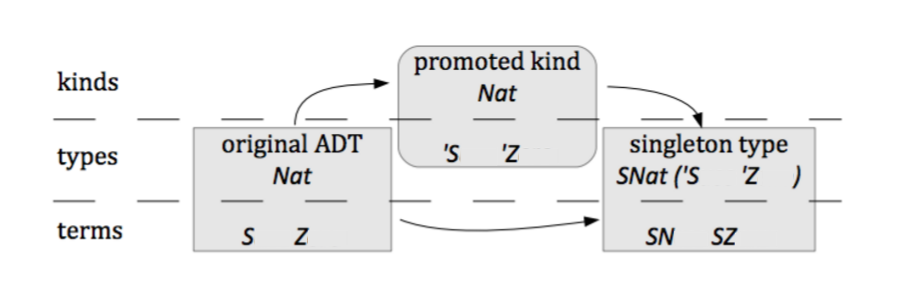
\includegraphics[width=\textwidth]{singleton.png}\label{singletonImg}

We can think of the DataKinds extension as a way of embedding dynamic information into the static fragment of the language. Singletons, on the other hand, are a way to reflect this static information back to the dynamic level, and make run-time decisions based on the types we obtain.

Singletons solve the two problems outlined above: they have kind \mintinline{haskell}{*} and contain a \mintinline{haskell}{Nat} that we can later refer to in the function type. We can now define \mintinline{haskell}{split} as follows:

\begin{minted}{haskell}
split :: SNat n -> Vec x (n :+ m) -> (Vec x n, Vec x m)
split SZ     xs          = (Vn, xs)
split (Sn n) (x `Vc` xs) = (x `Vc` ys, zs)
  where
    (ys, zs) = split n xs
\end{minted}

With these three tricks up our sleeve (data kind promotion, type level functions and singletons) we can emulate some of the features that are present in dependently typed languages such as Agda. These features allow us to emulate explicit dependent quantification. We can actually go even further in Haskell: Lindley et McBride \cite{hasochism} show us how to emulate implicit types via type classes and ultimately how all kinds of quantification, modulo some boilerplate, are possible in Haskell.

\subsection{Sum of Products}\label{SOP}

The basic idea of the Sum of Products (SOP) approach is to define a ``normal form'' for all generic representations of data types and 
to define generic functions by induction on this form. It is, in some sense, similar to the Disjunctive Normal Form for propositional logic in the sense that every proposition can be expressed in DNF and we can write theorems (functions) which assume the expression is represented in DNF.
The bulk idea is to view each type as a choice between a constructor and all the arguments that are passed to that constructor. It is useful to think about the two different levels: on the first level we make a choice about which constructor to pick; this corresponds to a sum
over all the constructors of the type. On the second level, we are choosing a certain number of arguments to feed to that constructor and this can be viewed as a list, or product, of 
those arguments. Clearly the products will depend on the choice of constructor, 
each of which could take a different number of arguments of possibly 
different types. This motivates the need to represent the product as some sort 
of heterogeneous list. A constructor can also take no arguments, in which case we 
can simply use an empty list to represent that, but can also take an argument of the same type it is trying to construct (like the \mintinline{haskell}{S} constructor from the previous section). 
In this case, the recursive argument can itself be encoded as an SOP and the same encoding can be used all the way down to the leaves. 

Since every data type can be encoded as an SOP, we can write functions 
that act on this representation. For each data type 
we can first convert it to the SOP representation and then pass it to 
the desired function. Since the SOP representation is isomorphic to the original type, we can eventually reconstruct the 
desired term after we are done working with the representation. This encoding is 
presented by Loh et al. \cite{true-sop} and represents one of the numerous different ways to 
approach generic programming in Haskell. 
In the remainder of this section we will try to formalize the intuition presented 
above by building the SOP representation of a data type. 

\subsection{Building our Universe}\label{universe}

An AST consists of a family of data types, with a main one which
represents the outer structure of the language, and a number of other
possibly mutually recursive data types appearing as arguments to the
constructors of the main data type. We can define a very simple language which 
consists of only one data type, \mintinline{haskell}{IntTree} which is isomorphic to binary trees 
of integers. This choice is just for ease of presentation, the following construction 
can be applied to a family of mutually recursive data types.

\begin{minted}{haskell}
data IntTree = Node IntTree IntTree | Leaf Int
\end{minted}

For each type that appears as an argument to a constructor in our family
of data types, we will construct an atom representing that type.
Following the example above, we will define

\begin{minted}{haskell}
data U = KInt | KIntTree 
\end{minted}

Now, we can group all the constructors appearing in our original
data types under the \mintinline{haskell}{Constr} type in a similar way as we
did for the atoms. 

\begin{minted}{haskell}
data Constr :: * where
  CNode :: Constr
  CLeaf :: Constr
\end{minted}

We have now deconstructed our original data type into two levels: \mintinline{haskell}{Constr} corresponding to the level of sums (the constructor) 
and  \mintinline{haskell}{U} corresponding to the level of products (the atoms).
\\
Since we had to define two additional data types that have no relation between 
each other we need a way to tie them together on the type level.
To achieve this, we define the \mintinline{haskell}{ConstrFor} data type,
which can be viewed as a proof that a certain constructor builds element
of a certain family. In general an AST consists of a family of possibly 
recursive data types, hence we will need the additional information about what 
family the constructor \mintinline{haskell}{Constr} belongs to.

\begin{minted}{haskell}
data ConstrFor :: U -> Constr -> * where
  NodeProof :: ConstrFor KIntTree CNode
  LeafProof :: ConstrFor KIntTree CLeaf
\end{minted}

Finally we must encode one last bit of information: the ``shape'' of
each constructor. To do so, we can use a closed type family which can be
viewed as a function on types. This function takes a \mintinline{haskell}{Constr} and
returns a list of atoms representing the arguments the constructor
accepts.

\begin{minted}{haskell}
type family TypeOf (c :: Constr) :: [U] where
  TypeOf CNode = '[KIntTree, KIntTree]
  TypeOf CLeaf = '[KInt]
\end{minted}

We will also need to associate each atom with a singleton, which will
allow us to relate terms of our language to their type level representation. 

\begin{minted}{haskell}
data Usingl :: U -> * where
  UInt :: Int -> Usingl KInt
  UIntTree :: IntTree -> Usingl KIntTree
\end{minted}

Since \toHaskell{TypeOf} returns something of kind \toHaskell{[U]} we will define another GADT named \toHaskell{All}, that maps a type constructor \toHaskell{k -> *} over an argument of kind \mintinline{haskell}{[k]} giving us something of kind \mintinline{haskell}{*} to quantify over a list of singletons.
\\
The definition for \mintinline{haskell}{All} is straightforward:

\begin{minted}{haskell}
data All (k -> *) :: [k] -> * where
  An :: All p '[]
  Ac :: p x -> All p xs -> All p (x : xs)
\end{minted}


With this setup we can finally construct the \mintinline{haskell}{View} data type; this loosely corresponds to a generic view as sum of products of a data-type, and simply deconstructs each term of a type into a constructor and a list of arguments applied to that constructor

\begin{minted}{haskell}
data View u where
 Tag :: ConstrFor u c -> All Usingl (TypeOf c) -> View u
\end{minted}

An element of type \mintinline{haskell}{View u} represents an element of type \mintinline{haskell}{u}  deconstructed into its SOP view; the first argument records the choice 
of the constructor for that datatype and the second is the heterogeneous list of 
arguments that are required to build that constructor, note that we are 
dependently relating the shape of the product to the actual choice of 
constructor (the \emph{c}).
\\
Finally, we want to define a pair of functions that allow us to move from an \toHaskell{Usingl} to a \toHaskell{View} and from that, back to the singleton representation.
\\
The \toHaskell{view} function, defined only for the recursive elements of the language can be implemented as follows.

\begin{minted}{haskell}
view :: IsRecEl r => Usingl r -> View r
view (UIntTree t) = viewTree t

viewTree :: IntTree -> View KIntTree
viewTree (Node t1 t2) = Tag NodeProof (UIntTree t1 `Ac` UIntTree t2 `Ac` An)
viewTree (Leaf i)     = Tag LeafProof (UInt i `Ac` An)
\end{minted}

We parametrize this function by the \toHaskell{IsRecEl} constraint, as atomic elements can not be deconstructed into a pair of constructor and arguments.
\\
The same holds for the inverse function \toHaskell{inj}: it will take as arguments the constructor, the list of arguments for that constructor and produce the corresponding \toHaskell{Usingl}.

\begin{minted}{haskell}
inj :: IsRecEl r => ConstrFor r c -> All Usingl (TypeOf c) -> Usingl r
inj NodeProof (t1 `Ac` t2 `Ac` An) = UIntTree (Node (UIntTree t1) (UIntTreet2))
inj LeafProof (i `Ac` An) = UIntTree (Leaf (UInt i))
\end{minted}

In the next section we will show the implementation of the type-directed diff. Our functions will operate on the concrete type \toHaskell{Usingl u} which we have shown how to instantiate.
It is worth noting that to achieve full-generality we could represent \toHaskell{Usingl} as a type-class instead of a concrete type. This would allow us to keep the implementation of the algorithm generally extensible as to new data-types other that the ones we mention it would suffice to give their \toHaskell{Usingl} instance. 
Techniques for lifting the concrete singleton data-type to a type-class are well-known and they were first showed by Eisenberg et al. \cite{singletons}. 
Since investigating the performance across different languages was never in the scope of this thesis, the code and the presentation are tied to the concrete \toHaskell{Usingl u} data-type.
%TODO Insert example of small generic function. Do we really need this? The next section is going to introduce examples of this. I feel like the important part here is the view.

\section{Type-directed diff}\label{type-directed-diff}

The approach presented by Miraldo, Swierstra and Dagand \cite{type-directed-diff} takes advantage of the structure encoded in types to define a generic type-directed diff algorithm between typed trees. 
The inspiration comes from the diff utility present in Unix; it is at the heart of the current methodologies employed by VCS to attempt to compute a patch between two different versions of the same file. 
The limitations of the diff algorithm, as it currently stands, is that it does not employ any structural information about the data on which it is trying to calculate a patch. 

The underlying idea to the approach presented in the article is to employ
the generic SOP view presented to obtain a view of any well defined program as a structured tree of data.  
We then try to compute a transformation, from one tree to the other, that respects the structural information we acquired.

In the process of transforming one tree into another we need to keep track of three different things: 
\begin{itemize}
  \item Transformations between constructors -- These are transformation between internal nodes of the trees.
  \item Transformations on the product level -- When transforming an internal node to another, we might end up in the situation where the nodes have a different number of children. We somehow have to align the children of the source node with the destination.
  \item Transformation between atoms -- The atoms can be either other internal nodes, in which case we recurse down the tree, or leaves in which case we record the pair of source and target leaf.
\end{itemize}

We will use the simple binary tree language presented in previous sections as a 
working example to show the construction of a patch. The transformation we will walk through is the following:
given the following AST:
\begin{minted}{haskell}
t1 = Node (Leaf 1) (Node (Leaf 1) (Leaf 1))
\end{minted}
we want to characterize the patch that transforms it to 
\begin{minted}{haskell}
t2 = Node (Leaf  1) (Node (Leaf 2))
\end{minted}

The first structure we will employ is the \emph{spine}, this can be thought of as a common skeleton between 
the two trees which captures the parts that do not change under the transformation.

\subsection{Spine}\label{spine}

We will define Spines only between two elements of the same sum-type, and defer to later the discussion on how
to perform transformation between elements of different sum-types. Calculating a spine for two elements of the same sum-type 
loosely corresponds to calculating the longest common prefix between two strings. Recall that the two 
elements \emph{x} and \emph{y} are viewed as SOP, in this sense calculating the
spine between \emph{x} and \emph{y} corresponds to capturing the common
co-product structure between them. Let $x$ and $y$ be two such elements, we will have three cases to
consider. 
\begin{itemize}
  \item $x = y$
  \item $x$ and $y$ have the same constructor on the sum level but differ in the 
  arguments
  \item $x$ and $y$ have different constructors
\end{itemize}

This gives rise
to the following three different constructors for the Spine GADT, each
corresponding to one of the cases described above.

\begin{minted}{haskell}
data Spine (at :: U -> *)(al :: [U] -> [U] -> *) :: U -> * where
  Scp  :: Spine at al u
  Scns :: ConstrFor u s -> All at (TypeOf s) -> Spine at al u
  Schg :: ConstrFor u s -> ConstrFor u r
       -> al (TypeOf s) (TypeOf r)
       -> Spine at al u
\end{minted}

If the two
elements are the same, the spine is a copy. If the top level
constructors match, the spine consists of this information and a function to
transform the constructor fields pairwise. Lastly, if two constructors
don't match, the spine must record this and also contain a function to
transform the list of source fields into the list of destination fields.
\\\\
%TODO Explain Kind?
The \mintinline{haskell}{Scp} constructor corresponds to the first case, in which we need
to record no additional information other than the fact that the two
elements are equal. 
Before looking at the other two constructors, let us focus our attention for a moment to the three arguments that a spine takes:
the third parameter of the spine (the \mintinline{haskell}{U}) represents the
underlying type for which we are trying to compute a patch, the sum-type to which $x$ and $y$ both belong.
The other two, \mintinline{haskell}{al} and \mintinline{haskell}{at} are respectively a
function between products that describes what to do with the different
constructor fields and a function between atoms which describes what to
do with the paired fields in case we have the same constructor.
These functions are needed for the remaining constructors: the \mintinline{haskell}{Scns} constructor corresponds to the 
case where the constructor is left untouched but some of the arguments have changed.
For this reason its second argument consists of the predicate \mintinline{haskell}{at} applied to the list of arguments which describes
how to transform them. 

Finally, \mintinline{haskell}{Schg} represents a change of constructor on the sum level: the first two arguments record the
source and destination constructors, the third argument is the
\mintinline{haskell}{al} function applied to the constructor fields of the source and
destination constructor respectively.

Let's not worry about the \mintinline{haskell}{al} and \mintinline{haskell}{at} parameters for the time 
being, these will later be used to close the recursive knot and generate the full patch by interleaving
the construction showed here and in the following sections. 
For now we can simply observe that if we were to calculate a spine between the 
two programs introduced above we would proceed by constructing their view as 
presented in \ref{SOP} obtaining the following

\begin{minted}{haskell}
v1 = Tag NodeProof (UIntTree (Leaf 1) `Ac` UIntTree (Node (Leaf 1) (Leaf 1)))
v2 = Tag NodeProof (UIntTree (Leaf 1) `Ac` UIntTree (Leaf 2))
\end{minted}

These views are not completely equal, but their first argument is. This represents the outer choice 
of constructor and we are after all ultimately transforming an \mintinline{haskell}{Node} into another one. The spine produced
by these two views will then start with an \mintinline{haskell}{Scns} recording the fact that 
the outer constructor has stayed the same but there are some changes in its 
arguments.

\begin{minted}{haskell}
spine = Scns NodeProof _
\end{minted}

We ignored the second argument up to this point (representing it as an underscore); let's turn our attention to 
that now: since we know that the constructor is unchanged in the transformation, we also know that 
both for the source and destination tree, the number and types of its arguments 
will be the same. For this reason we can simply pair up the corresponding 
arguments and calculate the diff between every pair. The second argument to \mintinline{haskell}{Scns} can be read as: the function 
\mintinline{haskell}{at} applied to a list of pairs of elements of the same type. The type of each 
pair is specified by \mintinline{haskell}{TypeOf s}, which in our working example is equal to 
\toHaskell{[KIntTree, KIntTree]}. Essentially we have a list of \mintinline{haskell}{UIntTree} pairs and are left with the problem of calculating patches between the elements contained in 
each pair. 
We can easily see that the first pair of our example will give rise to an \mintinline{haskell}{Scp}, the two sub-trees are in fact the same and we can simply copy the information along the transformation. 
The second pair is more interesting though: this is the case where we have a change on the constructor level and the spine we produce will be the following

\begin{minted}{haskell}
  Schg NodeProof LeafProof _
\end{minted}

However the remaining argument to fill is not as simple as the \mintinline{haskell}{Scns} case since \mintinline{haskell}{Node} and \mintinline{haskell}{Leaf} expect completely different 
arguments.
In the case where the constructor had remained the same, we could 
pair up the arguments and proceed from there; however, when the
external constructor has changed, there is no obvious way of pairing up
the arguments. Indeed they might be completely in different numbers and types, which 
motivates the following definition of alignments.

\subsection{Alignment}\label{alignment}

The spine takes care of matching
the constructors of two trees, alignments handle the products packed within the constructors.
Recall that this alignment has to work between two heterogeneous lists
corresponding to the fields associated with two distinct constructors.
The approach presented below is inspired by the existing algorithms
based on the edit distance between two strings. The problem of finding
an alignment of two lists of constructor fields can be viewed as the
problem of finding an edit script between them. An edit script is
simply a sequence of operations which describes how to change the source
list into the destination. In the case of \diff the source and destination lists are the lists of lines in the source and destination files; in our context
the source and destination lists are the products of fields of the source and destination constructors respectively. 
To compute an edit script we simply
traverse the lists, from left to right, considering one element from each
list. At each step we are presented with three choices:

\begin{itemize}
\item
  We can match the two elements (\amod) of the list and continue
  recursively aligning the rest
\item
  We can insert the destination element before the current element in
  the source list (\ains) and recursively compute an alignment between
  whatever we have in the source list and the tail of the destination.
\item
  We can delete the element from the source list (\adel) and recursively
  compute the alignment between the rest of the source and the
  destination.
\end{itemize}

The following GADT models the sequence of operations that represent an 
alignment.

\begin{minted}{haskell}
data AL (at :: U -> *) :: [U] -> [U] -> * where
  A0   :: Al at '[] '[]
  Ains :: Usingl u -> AL at xs ys -> AL at xs (u : ys)
  Adel :: Usingl u -> AL at xs ys -> AL at (u : xs) ys
  Amod :: at u -> AL at xs ys -> AL at (u : xs) (u : ys)
\end{minted}

\mintinline{haskell}{AL} is parametrised by the same type-level function introduced in the spine. 
\mintinline{haskell}{A0} represents the empty alignment, \mintinline{haskell}{Ains} and \mintinline{haskell}{Adel} take as first argument
a singleton representing the element being inserted or deleted. These two, together
with an alignment for the rest of the list, give us the alignment with
an insertion (resp. deletion) as explained in the section above. In the
\mintinline{haskell}{Amod} case the first argument is the predicate on the underlying atom that describes how to transform 
it and the second one, as for the case of insertions and deletions, represents an  
alignment between the rest of the lists. 
\\
One key difference to keep in mind, between the edit scripts produced by diff and the alignments is the atomicity of the elements being aligned (lines and sub-trees respectively). In the
case of strings we can assume deletions and insertions to be somewhat
equivalent in cost thus we can safely try to minimize one of the two.
However, in our case, the elements we are inserting or deleting are
sub-trees of arbitrary size, therefore it is not obvious if we should try and prune
insertions or deletions.
\\
This poses the problem that when enumerating alignments we have no guiding heuristic to cut the number
of solutions, for the time being we will simply ignore the problem and resort to enumerate
all possible alignments, to not skew the algorithm into preferring
insertions over deletions or viceversa.

Let's walk through calculating the alignment for our running example: we have to 
produce an alignment between \mintinline{haskell}{[KSExpr, KSExpr]} and \mintinline{haskell}{[Kint]} (recall that these are the shapes of the 
\mintinline{haskell}{Node} and \mintinline{haskell}{Leaf} constructors). Because of the way we 
define the \mintinline{haskell}{Amod} constructor, more precisely because of the \mintinline{haskell}{at} 
function that describes how to transform an atom into the other, we restrict 
ourselves to only attempt an \mintinline{haskell}{Amod} between two singletons of the same underlying type. 
\\
This means that in a case like this one, we will only be able to transform 
one list into the other by repeated applications of \mintinline{haskell}{Ains} or 
\mintinline{haskell}{Adel}. It is worth noticing that this restriction is not mandatory and 
we could in principle allow these transformations as well, the choice here is purely pragmatical and the underlying reason is,
this will be a recurring theme, to reduce the sheer amount of combinations that must be checked.
What we are left with are the three possible alignments that can be formed by inserting the \mintinline{haskell}{Uint} and deleting the two \mintinline{haskell}{UIntTree}s, we will generate all of them. 

\subsection{Atoms}\label{atoms}

Having figured out all the alignments between two lists of constructor
fields, we still have to decide what to do in the case where we match two
elements. We need to make a distinction between the possibly
recursive fields and the constant ones.
In the case of constant fields
like \mintinline{haskell}{Int}s or \mintinline{haskell}{String}s, a transformation between two
values of this type consists of a pair recording the source value and the
destination value. In the case of a recursive datatype we are
essentially left with the problem we started from: transforming a value
of a data type into another. To do so, we simply start all over again,
recursively computing a spine and an alignment between constructor
fields.
\\\\
To represent pairs of constant atoms we introduce a helper \mintinline{haskell}{Diagonal} datatype which 
lifts f over a pair of xs.

\begin{minted}{haskell}
newtype Diagonal (f :: k -> *) (x :: k) 
  = Diagonal { unDiag :: (f x , f x) }
\end{minted}

To distinguish between recursive and non recursive elements of the language we 
define a typeclass with no additional methods, and add instances of this typeclass only for the recursive atoms.
\\
Once again, borrowing the language definition from the previous section, we will have the following 
class and instances defined
\begin{minted}{haskell}
class IsRecEl (u :: U) where
instance IsRecEl KSExpr where
\end{minted}

With this we can define the following datatype to represent diffs between atoms of our language.
\begin{minted}{haskell}
data At (recP :: U -> *) :: U -> * where
  Ai :: (IsRecEl u) => recP u -> At recP u
  As :: Diagonal Usingl u -> At recP u
\end{minted}

Here the \mintinline{haskell}{At} datatype is parametrised by a predicate that describes how 
to transform the recursive atoms. 
The first constructor, \mintinline{haskell}{Ai}, which represents the recursive case is 
parametrised by this predicate, the constraint is added to ensure by construction 
that when we build an \mintinline{haskell}{Ai} we can only do so for the elements of the 
language that actually are recursive.
The other case is covered by the \mintinline{haskell}{As} constructor, recall that in this case \mintinline{haskell}{Diagonal} simply lifts 
\mintinline{haskell}{Usingl} to a pair of elements of type \emph{u}, so the first parameter 
can be read as: a pair of \mintinline{haskell}{Usingl u}.
\\
In our example we have already seen the case for \mintinline{haskell}{Ai}, the atoms paired 
by the first spine were all \mintinline{haskell}{Kexpr}s which we recursively calculated spines on. 
The \mintinline{haskell}{As} will be produced when we match two \mintinline{haskell}{Leaf}s that contain 
different integers, in that case we produce a pair of \mintinline{haskell}{Usingl Kint} that record 
the transformation from one \mintinline{haskell}{Int} to the other.

\subsection{Recursive alignments}\label{recursive alignments}

Starting by computing the spine is not necessarily the optimal choice, this can 
be seen from the following simple example between lists:

\begin{minted}{haskell}
  [ 1, 2, 3, 4 ] -> [ 2, 3, 4 ]
\end{minted}
Clearly the optimal patch will proceed to delete the first element and then 
copy over any remaining one. Our definition, however, does not allow for such 
deletions. Deletions (resp. insertions) are only handled by alignments. To 
handle such cases we can extend our spines and alignments with the datatype 
\mintinline{haskell}{Almu} that allows insertions or deletions to happen on the sum level.
\\
A match of constructors will be represented as a spine while insertions and 
deletions will record the constructor being inserted (resp. deleted) and a 
\mintinline{haskell}{Ctx} which records which fields are associated to that constructor.
\mintinline{haskell}{Ctx}s are inspeired by Huet zippers \cite{zippers}: they can be thought as a representation 
of a type with a hole somewhere; the hole represents the place where we 
plug in the rest of the tree to continue the computation.

\begin{minted}{haskell}
data Ctx (r :: U -> *) :: [U] -> * where
  Here :: (IsRecEl u) => r u -> All Usingl l  -> Ctx r (u : l)
  There :: Usingl u -> Ctx r l -> Ctx r (u : l)
\end{minted}

The \toHaskell{Here} constructor represents the hole, or the recursive position in which we want to carry on the computation. 

With this definition of contexts, we can finally define \toHaskell{Almu u v}, the datatype that represents structured patches between \toHaskell{u} and \toHaskell{v}

\begin{minted}{haskell}
data Almu :: U -> U -> * where
  Alspn :: Spine (At AlmuH) (AL (At AlmuH)) u -> Almu u u
  Alins :: ConstrFor v s -> Ctx (AtmuPos u) (TypeOf s) -> Almu u v
  Aldel :: ConstrFor u s -> Ctx (AtmuNeg v) (TypeOf s) -> Almu u v
\end{minted}

The \toHaskell{AlmuH}, \toHaskell{AtmuPos} and \toHaskell{AtmuNeg} are wrappers around \toHaskell{Almu}s to make source and destination types line up correctly.
\\
This gives rise to another occasion for non-determinism, as \mintinline{haskell}{Almu} has 
the same shortcomings of \mintinline{haskell}{AL} meaning that we have no obvious choice of 
what operation should be maximized over the others. As for alignments we decide to proceed non-deterministically
and compute every possibly choice. 

\subsection{Putting everything together}\label{putting everything together}

Now that we have defined all the types we need to represent our patches we are ready to define a function that given two \toHaskell{Usingl u} and \toHaskell{Usingl v} produces an \toHaskell{Almu u v} -- a patch that describes how to transform an \toHaskell{u} into a \toHaskell{v}.
We can write this function from the ``bottom up'', starting from the atoms and working our way up through spines and recursive alignments. 
\\
Notice how all these functions return a list of results, as non-determinism comes into play at every step. The signatures have been slightly simplified from the actual implementation where, for example, the result is parametrised by a monad, making it more general.
\\
We will only present the signatures of the functions in this section as it allows us to simplify some details of the implementation. The bodies of each function will be replaced by a short description which, given the types introduced up to this point and the supplied signature, will hopefully make it easy to fill in the gaps. 
The diff function for atoms should have the following signature
\begin{minted}{haskell}
  diffAt ::  (forall r . IsRecEl r => Usingl r -> Usingl r -> [rec r])
            -> Usingl a -> Usingl a -> [At rec a]
\end{minted}
This function is parametrised by a function that describes the treatment for 
recursive atoms. By inspecting the first singleton we learn whether the atom is 
recursive or not; if that is the case, the function that deals with the 
recursive elements can be used to build the corresponding \mintinline{haskell}{At}. In the 
other case, when the element is non recursive, we can simply pair up the two 
constant atoms with a \mintinline{haskell}{Diagonal} and build the non-recursive \mintinline{haskell}{At}.
\\
We need to define a function that given a pair of singletons produces all the spines between those two singletons. Remember that spines are parametrised by the alignment that handles the product structure, for this reason we will end up with as many spines as the number of alignments we need to consider.
\\
%TODO Define spine -> we need trivial alignment -> We need TrivialA, TrivialP (this is only one so we produce a single spine from this). Then we define align 
%align :: All Usingl p1 -> All Usingl p2
%      -> [ (Al TrivialA p1 p2, Int) ]
We can then proceed by implementing the function that computes all the spines 
between recursive elements.
\begin{minted}{haskell}
 diffS :: IsRecEl a => (forall r . IsRecEl r => Usingl r -> Usingl r -> [rec r])
        -> Usingl a -> Usingl a -> [Spine (At rec) (AL (At rec)) a]
diffS diffR s1 s2 =
       mapSpineM (uncurry diffAt . unContract)
            (uncurry $ alignP diffR) 
            (spine s1 s2)
  where
    alignP :: (forall r . IsRecEl r => Usingl r -> Usingl r -> [rec r])
           => All Usingl s -> All Usingl d ->  [AL (At rec) s d]
    alignP diffR p1 p2 = do
      al <- lift $ align p1 p2
      (mapAlM (uncurry diffAt . unContract) al)
\end{minted}

\mintinline{haskell}{diffS} lifts the parameter it takes, a function to handle the 
recursive elements of our language, over the predicate parameters to the spine that results from the two singletons.
%TODO Explain how we produce a single spine with trivial alignment, all the alignments with align ->  then use mapSpineM and mapAlM to produce the list of spines
We finally have to define a function that computes the diff in terms of 
\mintinline{haskell}{Almu}s. This will call \mintinline{haskell}{diffS} in case of two matching constructors from which we can compute the spine wrapping that with the corresponding \mintinline{haskell}{Alspn} constructor. In the other cases it will attempt the insertion (resp. deletion) at the constructor level by recording the constructor being inserted (deleted) and producing a \mintinline{haskell}{Ctx} which describes where the original tree is attached in respect to the added (deleted) constructor.
This function will have the following signature

\begin{minted}{haskell}
  diffAlmu :: (IsRecEl u, IsRecEl v) => Usingl u -> Usingl v -> [Almu u v]
\end{minted}

As is the case for the alignment between products, here we will simply proceed 
by enumerating all possible recursive alignments, attempting at each level 
the alignment of spines, insertions and deletions.
One shortcoming of this approach lies in the great combinatorial explosion of possibilities that arises in computing the alignments for constructors and products. We will see in the next sections what we will employ different techniques to keep this in check. 

\subsection{Applying Patches}\label{app_patches}

Now that we have constructed these type-safe patches we can define how to apply 
them to an expression to produce a transformed expression.

Application will be defined between a patch of type \mintinline{haskell}{Almu u v} and a 
singleton \mintinline{haskell}{Usingl u}. 
Again, we will proceed defining our functions from the atoms all the way up to 
recursive alignments. As before, our functions will be parametrised by one or 
more functions to deal with the recursive elements. 

\begin{minted}{haskell}
applyAt :: (IsRecEl a => rec a -> Usingl a -> Maybe (Usingl a))
        -> At rec a -> Usingl a -> Maybe (Usingl a)
applyAt appRec (Ai r) x = appRec r x
applyAt appRec (As c) x = if old == new then pure x
                          else if old == x then pure new
                          else Nothing
    where (old, new) = unDiag c  
\end{minted}

If we are dealing with a recursive element we can apply the supplied function 
and proceed the recursive application with that.
If the element is non-recursive, we check if it is a copy, in which we can 
return whatever argument we got. If it is a change instead, we will check if the 
argument matches the source and return the target.

Alignments will be applied to heterogeneous list of \mintinline{haskell}{Usingl u}. The function is parametrised by the previous function we defined over atoms.

\begin{minted}{haskell}
applyAl :: (forall a . at a -> Usingl a -> Maybe (Usingl a))
        -> AL at p1 p2 -> All Usingl p1 -> Maybe (All Usingl p2)
applyAl appAt A0 An
  = pure An
applyAl appAt (Amod p a) (Ac x xs)
  = Ac <$> appAt p x <*> applyAl appAt a xs
applyAl appAt (Ains k a) xs
  = Ac <$> pure k <*> applyAl appAt a xs
applyAl appAt (Adel k a) (Ac x xs) = do
  Refl <- testEquality x k
  applyAl appAt a xs
\end{minted}

Applying an alignment is straightforward, the types guarantee that we can only 
apply lists of \mintinline{haskell}{Usingl}s and alignments which are compatible. This is 
reflected by the fact that the supplied alignment has type \mintinline{haskell}{AL at p1 p2} 
which matches the type in \mintinline{haskell}{All Usingl p1} and the result produced by 
applyAl has type \mintinline{haskell}{All Usingl p2}. We step through the alignment applying 
each \mintinline{haskell}{AL} to the head of the list until we are done.

\begin{minted}{haskell}
  applyS :: IsRecEl r => (forall a . at a -> Usingl a -> Maybe (Usingl a))
       -> (forall p1 p2 . al p1 p2 -> All Usingl p1 -> Maybe (All Usingl p2))
       -> Spine at al r
       -> Usingl r
       -> Maybe (Usingl r)
applyS appAt appAL Scp x = pure x
applyS appAt appAL (Schg i j p) x = case view x of
  Tag c d -> do
    Refl <- testEquality c i
    inj j <$> appAL p d
applyS appAt appAL (Scns i p) x = case view x of
  Tag c d -> do
    Refl <- testEquality c i
    inj i <$> sAll appAt p d
\end{minted}

Application for spine is parametrised by a function to apply atoms and one to 
apply alignments. We inspect the spine and proceed accordingly. If it is an \scp 
we return the argument, if it is an \schg we need to inspect the argument and 
convert it to the SOP view. If the constructor on the sum level matches the 
source constructor of the \schg then we can construct the element with the 
target constructor and the result of the application on the alignment.
Finally, if the constructor is an \scns, we start by peeling the argument and 
turning it into its SOP view. If the constructors match, then we can construct 
the element with the old constructor plus the result of applying \mintinline{haskell}{appAt} 
to every pair of atoms found by pairing the product in the \scns and the view of 
\mintinline{haskell}{x}.

Finally, for the case of recursive elements, we can give the following 
implementation.

\begin{minted}{haskell}
applyAlmu :: (IsRecEl u, IsRecEl v) => Almu u v -> Usingl u -> Maybe (Usingl v)
applyAlmu (Alspn s) x = applyS (applyAt applyAlmu) (applyAl (applyAt applyAlmu)) s x
applyAlmu (Alins constr ctx) x = inj constr <$> ctxIns ctx x
applyAlmu (Aldel constr ctx) x = case view x of
  (Tag c1 p1) -> do
    Refl <- testEquality constr c1
    ctxDel ctx p1
\end{minted}
% Highlighting is broken :/ $

The case of \alspn amounts to simply calling the function we have defined to 
apply spines with the correct arguments.
In case of an \alins, we still have to construct an element, it will be obtained
by an injection of the inserted constructor and the context. 
\mintinline{haskell}{ctxIns} walks through the context collecting all the singletons and 
calling the application recursively when it finds the hole.
In case of a deletion, we don't have to build anything. We check if the element 
matches the constructor we intend to delete and simply carry on if it does.
\mintinline{haskell}{ctxDel} walks through the context, throwing away every singleton it 
finds and only calling the recursive application once it finds the corresponding 
hole.

\subsection{Disjointedness}\label{disj}

We can define a predicate to decide disjointedness between patches. We want to define this notion only for pair of patches that share the same source, as patches from completely different sources are incomparable to each other. 
The idea that we want to capture with disjointedness is that two disjoint patches should always commute; this means that we can apply them in any order to the source and always get the same result.

We can start by attempting to define what disjointedness is on the recursive 
level.  Disjointedness should model the fact that two patches are acting on different parts of the source. This suggests we want to impose the condition that any patch different from the trivial one, is disjoint from itself.  
\\
Following this line of though we can start by defining

\begin{minted}{haskell}
disjointAlmu _ _ (Alins _ _) (Alins _ _) 
  = False
disjointAlmu _ _ (Aldel _ _) (Aldel _ _)
  = False
\end{minted}

When matching an \alins with anything else, we extract the focus from the context, and recursively call the disjointedness predicate on the focus and whatever the other argument is. In other words, insertions are always allowed.

\begin{minted}{haskell}
disjointAlmu (Alins constr ctx) almu
  = disjointFromCtxPos ctx almu
disjointAlmu almu (Alins constr ctx)
  = disjointFromCtxPos ctx almu
\end{minted}

When we match an \aldel with an \alspn we will inspect the spine contained in the \alspn.
\\
If it is an \scp then the two are trivially disjoint.

\begin{minted}{haskell}
disjointAlmu _ _ (Aldel c ctx) (Alspn Scp)
  = True
disjointAlmu _ _ (Alspn Scp) (Aldel c ctx)
  = True
\end{minted}

If it is an \scns then they are disjoint if the recursive changes within the \scns do not change the deleted context and the focus of the context is disjoint from the corresponding changes in the \scns product.

\begin{minted}{haskell}
disjointAlmu  (Aldel c ctx) (Alspn (Scns c' ats))
  = case testEquality c c' of
      Just Refl -> disjointFromCtxNeg ctx ats
      Nothing   -> False
disjointAlmu (Alspn (Scns c' ats)) (Aldel c ctx)
  = case testEquality c c' of
      Just Refl -> disjointFromCtxNeg ctx ats
      Nothing   -> False
\end{minted}

If it is an \schg then they are not disjoint.

The only case left is when we have two \alspn. In this case we have to look at 
the pair of spines to decide if they are disjoint. 
As before, we can step through all the cases.

\scp is disjoint from any other node. 

\begin{minted}{haskell}
disjointS Scp s'
  = True
disjointS s'  Scp
  = True
\end{minted}

A pair of \scns is disjoint if the constructor they fix is the same and if their 
fields are pairwise disjoint.

\begin{minted}{haskell}
disjointS (Scns c p) (Scns c' p')
  = case testEquality c c' of
          Just Refl -> disjAts p p'
          Nothing   -> False
\end{minted}                   

A pair of \schg is never disjoint.


Finally, when we have an \scns and a \schg, they are disjoint if the constructor 
fixed by \scns is the constructor changed by \schg and if the fields of \scns 
are disjoint from the alignment in \schg. 

\begin{minted}{haskell}
disjointS disjointAt (Scns c p) (Schg i j p')
 = case testEquality c i of
         Just Refl -> disjAtAl p p'
         Nothing   -> False

disjointS disjointAt (Schg i j p') (Scns c p)
 = case testEquality c i of
         Just Refl -> disjAtAl p p'
         Nothing   -> False
\end{minted}

The predicate \toHaskell{disjAtAl} follows the same pattern outlined up to this point.
Since we learned that the constructor of \scns and the source constructor of \schg are the same we know that this alignment has as source exactly this list 
of fields. We can step through the elements considering them in pairs. 
Insertions are always fine as long as the rest of the patches are disjoint.
If we find an \adel we have to check that the patch on the field being deleted is actually and identity patch. 
Lastly, when the alignment contains an \amod we can check if the argument of the \amod is disjoint from the field.
\\
To do so we need to introduce a function that tells us when two atoms are disjoint, the recursive case can be dealt with a function which will be taken as the first argument to close the recursive loop.
Finally, two non-recursive atoms are disjoint if either one of them is the identity (represented by a pair containing the same element).

\begin{minted}{haskell}
disjointAt :: (IsRecEl a => rec1 a -> rec2 a -> Bool)
           -> At rec1 a -> At rec2 a -> Bool
disjointAt disjointR (Ai r) (Ai r') = disjointR r r'
disjointAt disjointR (As p) (As p')
  = old == new || old' == new'
  where
    (old, new) = unDiag p
    (old', new') = unDiag p'
\end{minted}

\subsection{Clojure}
Having developed a general framework to compute patches between typed trees, we know want explore its performance in the context of a real programming language.
To test this, we developed a parser for Clojure; the implementation of this parser can be somewhat different to one designed to interpret and run Clojure code, this is because in this context we are more concerned with capturing the syntactical structure rather than the semantical one. One further consideration is that the parser should try to capture as much syntactical information as possible, in order to produce code that strives to respect any syntactical convention embraced by the authors.

The AST will be composed by a family of data-types, with the \toHaskell{Expr} type representing the "entry point" for each parse. 

\begin{minted}{haskell}
data Expr = Special FormTy Expr
          | Dispatch Expr
          | Collection CollType SepExprList
          | Term Term 
          | Comment String
          | Seq Expr Expr
          | Empty
          
data SepExprList = Nil
  | Cons Expr Sep SepExprList
 
data Term = TaggedString Tag String

data Sep = Space | Comma | NewLine | SEmpty
data FormTy = Quote | SQuote | UnQuote | DeRef
data CollType = Vec | Set | Parens
data Tag = String | Metadata | Var
\end{minted}

This is enough to parse all Clojure code obtained from the test data that we collected; it can actually parse even more than legal Clojure as it does not consider the semantical correctness of the parsed code, only its syntactical coherence. The definition of \toHaskell{SepExprList} can represent lists of expressions separated by either newlines, commas or spaces, which are all legal legal and interchangeable separators in Clojure, we also have an \toHaskell{SEmpty} separator for the \toHaskell{Nil} case.

We can apply the same procedure outlined before to generate the required singletons and type families. The only difference from before is that in this case is that our language is represented by a family of mutually recursive datatypes. If you recall from section \ref{dependent-types-in-haskell} we introduced \toHaskell{ConstrFor} to relate our singleton constructors to the type they were constructing. In case of a single data-type representing the whole AST there was no real necessity for this type, and we could have resorted so simply passing \toHaskell{Constr} around. In the case of the Clojure AST we need this additional information, and the \toHaskell{ConsrFor} type becomes (slightly) more interesting.

\begin{minted}{haskell}
data ConstrFor :: U -> Constr -> * where
  NilProof :: ConstrFor KSepExprList Nil
  ConsProof :: ConstrFor KSepExprList Cons

  SpecialProof :: ConstrFor KExpr Special
  DispatchProof :: ConstrFor KExpr Dispatch
  CollectionProof :: ConstrFor KExpr Collection
  TermProof :: ConstrFor KExpr Term
  CommentProof :: ConstrFor KExpr Comment
  SeqProof :: ConstrFor KExpr Seq
  EmptyProof :: ConstrFor KExpr Empty
  
  [...]
\end{minted}

As the constructor name suggests, we can think of these as proofs that  that a certain \toHaskell{Constr} maps to a specific \toHaskell{U}. These are straightforward to generate manually, but can also be generically derived.
\\
Finally we will have to add \toHaskell{IsRecEl} instances for the recursive elements of the family, we can define these instances for \toHaskell{Expr}, \toHaskell{SepExprList} and \toHaskell{Term} only, and treat all the other types as atoms.  



\section{Heuristics}

When moving from our toy language to a more complex one like Clojure, we soon run into the limitations of our non-deterministic approach.
Non-determinism sneaks in when we have to compute an alignment, either on the recursive or on the atomic level. 
\\ 
It is easy to see that in some cases, prioritizing deletions can be more profitable and in other it may be better to do the opposite; this uncertainty stems from the fact that at the time we are calculating the alignment we have no information about the size of the sub-trees we are considering. 
\\
Since we don't know a priori which alignment is more efficient, in the original specification we simply decide to enumerate all possible ones. This number can grow very quickly and, to make things worse, we are dealing with alignments of arbitrarily large subtrees, which prevents
us from optimising towards insertions or deletions.
\\
In this section we will define some heuristics we can use to guide this process of enumeration in order to trim down the amount of computations that need to be carried on.
\\
These heuristics fall under two categories.
\\
One is to explore the possibility of using the standard unix \mintinline{haskell}{diff3} algorithm as an oracle to prune the alignment trees that are being generated. 
The idea is that instead of enumerating all possible alignments between two trees, we can check and see how \diff3 treats the sequence of lines in which that tree resides in the source. This can allow us to prune the search space based on the information we can derive from \diff3 and may be able to speed up the computation to handle larger inputs. This idea can be taken a step further. We can generalise the approach to add an "Oracle" which, based on some internal state, generates the next branches that should be explored.
\\
We can define different Oracles and explore different strategies to reduce the combinatorial explosion. 
One of the upsides of this approach is that it will allow us to test different kinds of optimisations in a clean and flexible way; we could even imagine an oracle that interacts with the user, occasionally asking her for guidance into which branches to pursue. 
Furthermore, we could define a notion of composition between oracles that will give us the chance to combine different optimisations into one.
\\
Another approach that we could take in the attempt to speed up the algorithm is to define an heuristic to score patches which will allow us to greedily prune the search space. 
With this approach, the question that arises is: what are the properties of patches for which we can compare and score them? The answer is not clear yet. Informally we want to prefer patches that make minimal modifications and encourage copying as much as possible. This is because 
if a patch consists of a copy on a certain sub-tree, we can be sure that we can 
safely merge this with any patch that modifies that same sub-tree. 
In other words, want to define an heuristic that picks the patch that maximises the chances of it being disjoint from any other patch from the same source.
\\
\subsection{Basic Oracles}\label{oracles}
The goal for Oracles is to be able to have a uniform interface to implement different kinds of optimisations, heuristic and possibly even human interaction in the process of generating all the possible patches.
 \\
The key idea, is to extend the algorithm to perform a monadic action at each non-deterministic ``junction''. The result of this action will be a list that encodes which branches should be explored and which should be cut from the enumeration of patches.
\\
We can start by observing that in both places where we have a non-deterministic choice, we always have to pick between three possible paths: namely to insert or delete something or to match source and destination in a pair. We can model this with a very simple datatype

\begin{minted}{haskell}
  data Path = I | M | D 
\end{minted}

Where the three constructors respectively stand for: Insert, Modify and Delete.
We want to give our oracles the possibility to inspect the history of issued paths on each branch, this can be modeled with a reader monad.

\begin{minted}{haskell}
type HistoryM = ReaderT [Path]
\end{minted}

We can now define our Oracle class

\begin{minted}{haskell}
class Oracle o m where
  callP :: o -> All Usingl p1 -> All Usingl p2 -> HistoryM m [Path]
  callF :: (IsRecEl u, IsRecEl v) 
  	=> o -> Usingl u -> Usingl v -> HistoryM m [Path]
\end{minted}

The Oracle class has two functions, one for the choice on the constructor level and one for the choice on the product level. At each choice, the oracle has access to the history of paths issued on the branch via the history monad, and  has also access to it's internal state (the $o$ type).
\\
Notice that the signatures differ in the arguments they take, \toHaskell{callP} is meant to handle alignments on the product level, as such it takes the two heterogeneous lists that are being aligned. \toHaskell{callF} on the other hand, is meant to handle the recursive alignments on the constructor level and takes two singletons as input (the 'F' stands for fixpoint)
 
\subsubsection{NoOracle}
To warm up we can start by defining the "unit" oracle. 

\begin{minted}{haskell}
data NoOracle = NoOracle
instance (Monad m) => Oracle NoOracle m where
  callP _ An         An         = return []
  callP _ An         (_ `Ac` _) = return [I]
  callP _ (_ `Ac` _) An         = return [D]
  callP _ _          _          = return [I , M , D]

  callF _ _ _ = return [I , M , D]
\end{minted}

This oracle will not contain any global information and will ignore the history of issued paths. It will simply output all possible choices in any non-trivial case.

\subsubsection{NoDupBranches}

The first optimisation we want to encode is to limit the duplicate branches being explored: we avoid performing an insertion if the last step was a deletion and vice-versa.
It is easy to see that an insertion followed by a deletion is equivalent to a deletion followed by an insertion, furthermore -- if we can match two elements -- then the match will never be worst than an insertion followed by a deletion.
\\
We can define the following function that looks at the history of issued paths to avoid performing an insertion if the last step was a deletion and vice-versa. The last step is attached in front of the list as it is more efficient that traversing the list every time to add it at the end.

\begin{minted}{haskell}
nextPaths :: [Path] -> [Path]
nextPaths (I:_)     = [I, M]
nextPaths (D:_)     = [D, M]
nextPaths (M:_)     = [I, M, D]
\end{minted}

Given this function we can implement the \mintinline{haskell}{NoDupBranches} oracle

\begin{minted}{haskell}
data NoDupBranches = NoDupBranches

instance (Monad m) => Oracle NoDupBranches m where
  callP _ An         An         = return []
  callP _ An         (_ `Ac` _) = return [I]
  callP _ (_ `Ac` _) An         = return [D]
  callP _ (s `Ac` _) (d `Ac` _) = ask >>= return . nextPaths

  callF _ s d = ask >>= return . nextPaths
\end{minted}

\subsection{Oracle composition}

With the oracles we gain the possibility to tweak the run-time behaviour of the 
algorithm without have to change any parts of the actual implementation.
An advantage of this is that we can define a notion of 
composition between oracles; this way we can layer different processes, each of 
which is independent of the other in terms of implementation.
\\
The composition we define wants to model a stack of oracles, the oracles are 
interrogated in the order in which they appear on the stack. When an oracle is 
interrogated, only if the answer is an empty list we will go down the stack and 
ask the oracle underneath. 
\\
This means that we can build other optimisations on top of \mintinline{haskell}{NoDupBranches}, these optimisations can also be partial or based on heuristics, as long as we have a ``safe'' oracle at the bottom of the stack we can always fallback to the ones below in the cases when it is not clear which choice should be done.

\begin{minted}{haskell}
  data ComposeOracle a b = ComposeOracle a b

-- Give it a nice constructor
(<°>) :: a -> b -> ComposeOracle a b
a <°> b = ComposeOracle a b

instance (Monad m, Oracle a m, Oracle b m) => Oracle (ComposeOracle a b) m where
  callF (ComposeOracle a b) s d = do
    o1 <- callF a s d
    case o1 of
      [] -> callF b s d
      o1 -> return o1

  callP (ComposeOracle a b) s d = do
    o1 <- callP a s d
    case o1 of
      [] -> callP b s d
      o1 -> return o1
\end{minted}

\subsection{DiffOracle}
A considerable speedup can be obtained by using \diff to prune the 
search space. We can define a datatype, which mirrors the definition of a path 
and identifies which lines are copied, which are deleted and which are inserted 
according to \diff.

We will call this datatype \mintinline{haskell}{DiffAction} and it will have the following 
definition.

\begin{minted}{haskell}
  data DiffAction = 
    OMod LineRange LineRange
  | OIns LineRange
  | ODel LineRange  
\end{minted}

Where \toHaskell{LineRange} is a pair of \toHaskell{Int} which represent the first and last line of the corresponding region.
We can think of \toHaskell{DiffAction} as some sort of Edit Script, with the difference that in addition to copies, insertions and deletions we introduce modifications.
We will produce an \toHaskell{OMod} every time we have two contiguous regions of insertions or deletions between the source and destination file. The regions tagged by an \toHaskell{OMod} are the ones where we attempt to produce a more accurate patch than \diff. 
\\
Note that regions that are not covered by any \toHaskell{DiffAction} are implicitly considered copies.
\\
For example, given this pair of source and destination
\\
\\
\begin{minipage}[t]{0.5\textwidth}
\begin{minted}[linenos]{clojure}
  (defn function
    [a b]
    return a)
\end{minted}
\end{minipage}
\begin{minipage}[t]{0.4\textwidth}
\begin{minted}[linenos]{clojure}
  ;; A comment
  (defn function
    [a b]
    doSomethingElse
    return b)
\end{minted}
\end{minipage}
\\
\\
The preprocessing will produce the list \toHaskell{[OIns (1,1), OMod (3,3) (4,5)]}. The first line can be definitely ruled as an insertion, as it is adjacent to a copy on both the source and destination. \emph{Diff} records line 3 of the source as a deletion and lines 4 and 5 of the destination as insertions. This gives us two contiguous regions of insertions and deletions between source and destination and are accordingly recorded as a modification. 

Since traversing the whole list of \toHaskell{DiffAction} every time we want to call the oracle is not very efficient we can encode the same information in a pair of maps from \toHaskell{Int} to \toHaskell{Path} (one for the source and one for the destination files). 
\\
Given this pair of maps, the oracle will extract the \toHaskell{LineRange} contained in each \toHaskell{Usingl u} and lookup the line that corresponds to the beginning of the \toHaskell{LineRange} in the corresponding map. 

We can define the following helper predicate

\begin{minted}{haskell}
isMod :: LineRange -> M.IntMap Path -> Bool
isMod lr m = case M.lookup (takeStart lr) m of
  Just M -> True
  _      -> False
\end{minted}
and the corresponding \toHaskell{isIns} and \toHaskell{isDel} we can finally define the \toHaskell{giveAdvice} function.

\begin{minted}{haskell}
giveAdvice :: DelInsMap -> Usingl u -> Usingl v -> [Path]
giveAdvice (srcMap, dstMap) src dst =
  if (isMod srcRange srcMap && isMod dstRange dstMap)
    then []
  else if (isDel srcRange srcMap || isMod srcRange srcMap)
    then [ D ]
  else if (isIns dstRange dstMap || isMod dstRange dstMap)
    then [ I ]
  else [ M ]
  where
    srcRange = fromJust $ extractRange src
    dstRange = fromJust $ extractRange dst

\end{minted}

In case in which the ranges do not match with anything in our maps, we simply want to emit an \toHaskell{M}, as these expressions lie in lines that \diffthree identified as copies (we will see that this gives rise to some problems as \diff can copy in a way that our algorithm does not support). 
When both source and destination are marked as \toHaskell{OMod}, we are essentially in a range where we know that \diff can not reconcile the changes between source and destination  and will simply delete everything in the source and insert everything in the  destination. 
This is the case where we can attempt to generate a more efficient patch, so we return an empty list to fall back to any underlying oracle that will compute a full enumeration in that range. 
\\
Alternatively, if the source is marked as a deletion, or the destination is marked as an insertions, we will emit the corresponding instruction.
In the else cases we also check if either the source or the destination is marked as modification (but the other one isn't as the first check was already showed to be false at this point). We have to handle the case that when transforming a source into the destination, we end up on a branch that has inserted (resp. deleted) everything it had to, and it simply needs to delete (rep. insert) the remaining range.
\\
Finally, the full oracle can be defined as follows:

\begin{minted}{haskell}
instance (Monad m) => Oracle DiffOracle m where
  callF o s d = return (askOracle o s d)

  callP _ An         An         = return []
  callP _ An         (_ `Ac` _) = return [ I ]
  callP _ (_ `Ac` _) An         = return [ D ]
  callP o (s `Ac` _) (d `Ac` _) = return (askOracle o s d)

askOracle :: DiffOracle -> Usingl u -> Usingl v -> [Path]
askOracle (DiffOracle diffActions) src dst 
  = case (extractRange src, extractRange dst) of
      (Nothing, Nothing)         -> [ M ]
      (Just sRange, Nothing)     -> [ D ]
      (Nothing, Just dRange)     -> [ I ]
      (Just sRange, Just dRange) -> giveAdvice diffActions src dst
\end{minted}

We can exploit the fact that the \toHaskell{LineRange} is only defined for the recursive elements of the family, which means that in the case we can not extract it, we can short-circuit the computation since we never pair up non-recursive elements with recursive ones.

\subsubsection{Shortcomings}
One of the issues with this optimisation is that not every modification between source and destination file is correctly identified by this procedure. Some problems arise when changes in the resulting AST are invisible to diff. Suppose that we didn't include empty expressions in our AST and modeled the top-level parse as either a single expression or a sequence of multiple ones. 
What happens when try to compute the patch between the following files?
\\
\begin{minipage}[t]{0.5\textwidth}
\begin{minted}[linenos]{clojure}
(keep
  old keep)
\end{minted}
\end{minipage}
\begin{minipage}{0.5\textwidth}
\begin{minted}[linenos]{clojure}
(keep
  new keep)
(new new)
\end{minted}
\end{minipage}
\\
\\
The preprocessing will produce the following list of \toHaskell{DiffAction}:
\toHaskell{[OMod (2,2) (2,3)]}. 
However, to perform the optimal patch between these two programs we clearly want to insert a \mintinline{haskell}{Seq} on the first line and proceed calculating the diff from there. 
By following the \diff instead, we realize we had to change the external node when it is too late, we are already on line 2 and have already decided to copy over the first line. 
At its core, the problem lies in the fact that the external change is invisible to \diff, since it only deals with lines, and the addition of lines at the end does not influence in any way the lines at the beginning of the file. 
In our case, we have the whole expression tree, and adding a line at the end of the file does not necessarily only trigger changes on the leaves of the tree, but changes can bubble up to the root, as in the example shown.


\subsubsection*{Possible Solutions}
There are different ways we can solve this problem. 
One is to carefully think about which nodes have this "non-local influence" and treat them in a special way. 
For example, the problem presented in the previous snippet arises from the fact that -- when transforming a top level expression from a single \toHaskell{Expr} to a \toHaskell{Seq} -- we can only realize that this change has to be made when we get to the second \toHaskell{Expr}. 
Whenever we change a single expression to a sequence of two by adding one at the end, we will inevitably mark the first expression as a copy, and the second as an insertion. This means it will be ``to late'' when we get to the inserted line: we already decided to copy a node which leaves us no space to insert the new expression.
\\
\\
One solution is to design the AST in a way that prevents this problem from ever coming up. If we modelled the top-level of a program so that the top level is always a \toHaskell{Seq}, and we add an \toHaskell{Empty} constructor to \toHaskell{Expr} an example like the previous one, would not be problematic anymore. 
Indeed, when we get to the second line, we don't have to change the previous constructor anymore, as the source will conveniently contain an \toHaskell{Empty} expression slot in which we can insert our new expression.
This solution has the problem of being very ad-hoc. We have to modify the parser and add support for the new constructors throughout the implementation. Empty expressions turned out to be useful in any case, as we need them to model the patch that inserts into an empty file, but the solution is clearly not satisfactory as it requires us to model our AST in a very specific way which breaks our claim to generality.
\\
\\
A better solution would be to design oracles that can deal with the problematic cases. 
Sticking to the example presented earlier, we could define a simple oracle which ignores everything, except the case when it gets as input a single expression from the source and a sequence of multiple ones in the destination. In that case we know that -- no matter what the other oracles say -- we must insert a \toHaskell{Seq} node on the top-level; in that situation we can directly return \toHaskell{I} and skip the other oracles. 
\\
This solution is better than the previous one, as it is less invasive. It is still troublesome however that the correctness of the oracle depends on an oracle being present before it. Also, if we want to add support for other languages in the future we will have to carefully re-implement the ad-hoc oracles for the new languages. To solve these last lingering issues, we can adopt a different strategy. 
\\
\\
Ultimately the problem lies in the fact that there are two distinct actors at play: on one hand we have the AST, on the other the actual lines of code, which can be thought of as a pretty-printed representation of the AST. We are using the line based solution over the pretty-print of the AST to derive a solution on the AST. Our problems come from the fact that changes to the pretty-printed AST don't always map one-to-one to changes in the AST. If we could somehow run the line based diff on the AST directly there would be no discrepancies. To do so, we can print the AST to a file and, since every constructor is annotated with a line range which tell us on what line it appears, we can print each sub-tree on the lines the elements it contains appear in. 
We can now run \diff to preprocess the ASTs printed in this way. Each change that was detected by running on the original files will also be detected by looking at the ASTs, as they are representations of the content of those files. The converse, is not true though, by running \diff on the AST we know exactly on which levels of the tree, modifications on certain lines reflect.
The problematic case we showed earlier will now be correctly recognized. Indeed, by printing the ASTs of the two files showed earlier, we will immediately detect that on line 1 the constructor has changed from \toHaskell{Collection} to \toHaskell{Seq}.

\subsubsection{Further Shortcomings}

Another problem, perhaps even more troubling, is that \diff can mark some parts as copies even though these copies are illegal for our algorithm. 
Imagine a case where we have this pair of source and destination files
\\
\\
\begin{minipage}{0.5\textwidth}
\begin{minted}[linenos]{clojure}
((keep
  del
keep))
\end{minted}
\end{minipage}
\begin{minipage}{0.5\textwidth}
\begin{minted}[linenos]{clojure}
((keep
  ins)(
keep))
\end{minted}
\end{minipage}
\\
\\
In this case, according to \mintinline{haskell}{diff3} we are supposed to copy lines 1 and 3 
and modify line 2. The problem is that -- in the source file -- we have a \toHaskell{Cons} node 
that contains all the copied lines in one of its children. In the destination 
however, some of these lines are copied to the left child of a Cons, and others 
to the right. In the example above this can be seen on the \toClojure{keep} appearing on line 3, which will end up in a different expression than the one on the first line. 
What happens is that \diff3 can copy nodes across adjacent sub-trees, but our algorithm does not: we have to pick one of the two sub-trees and attempt the copies only into that.
\\
When we are transforming a \toHaskell{Cons} \toHaskell{a} \toHaskell{Nil} into a \toHaskell{Cons} \toHaskell{c} \toHaskell{d} the only option we have is to insert \toHaskell{d} in the place of \toHaskell{Nil}. 
However, according to \diff, lines in the sub-tree \toHaskell{a} get copied both to \toHaskell{c} and \toHaskell{d}. In practice this means that when we are at the step in which we have to calculate the patch between \toHaskell{a} and \toHaskell{c}, we are left with inconsistent information, in particular we marked some nodes as copies into \toHaskell{d} when we actually want to delete them.

\subsubsection*{Possible Solutions}

To solve this problem we must find a way of detecting when a situation like the 
one described above arises. We can formulate the problem as follows:
given the following source and destination nodes

\begin{minted}{haskell}
src = Seq a b
dst = Seq c d
\end{minted}


\begin{itemize}
  \item Let $CopyPairs(P)$ be the set of pairs $(s,t)$ that are marked as copies by \diff3 in the program $P$.

\item Let $CopySet(e)$ be the function that extracts all the lines marked as copies 
contained in an expression $e$ (A line is marked as copy if it appears in one of the pairs resulting from $CopyPairs(P)$).
\end{itemize}

Then, if we can find an $s \in CopySet(a)$ such that $t \in CopySet(c)$, where $(s,t) \in CopyPairs(P)$ and we can find $s' \in CopySet(a)$ such that $t' \in CopySet(d)$, where $(s',t') \in CopyPairs(P)$ then we know we are in a conflicting situation. 
\\
This condition deals with the case where we had to insert a sub-tree which 
contains at least one expression marked as copy, to deal with the deletion as well, we 
must also check that the converse condition does not hold going from $c$ to $a$ 
and $b$.
\\
Once we detected the conflicting copy across sub-trees, we can simply remove pairs from the set $CopyPairs(P)$ until the previous condition is satisfied. In other words, after we detect that a node contains copies over sub-trees, we pick one of the sub-trees and remove all the copies contained in it.
\\
\\
The only step that is still missing is about which criteria can be used to pair up the nodes we must check. 
One way to formulate the problem is the following: we run into this issue whenever we have a pair of candidate nodes that are marked as copy on their outer level (resulting in an \mintinline{haskell}{Scns} in our case), but would then later attempt to copy across subtrees.  
The crucial observation is that the candidate nodes to check will always start on a line that \diff will have marked as copies (this is exactly the issue, \diff can issue a copy there and move across sub-trees later, our algorithm can not). 
\\
\\
One solution could be to extend the oracles to add support for a \mintinline{haskell}{De-optimise} operation. The oracle should be able to perform some computation on each branch 
and decide if it should keep operating on subsequent computations that follow from that branch.
This could very well consist in performing the check we described earlier to detect when the information contained in the DiffOracle is not trustworthy anymore, and proceed the process ignoring the oracle which is marked as de-opt. 
Supporting this interface might be also very useful if we plan to write a human-interaction oracle, where we could have it work on the top levels of the tree (e.g. user matches top level expressions) and then turn off as the program takes care of the of the deeper levels. 
\\
\\
Another solution, could be to try and solve the problem with some preprocessing.
\\
This criteria identified to match nodes suggests an enumeration strategy that we could use to break any eventual conflicts in the \mintinline{haskell}{[DiffAction]}. 
The idea is to identify which lines \diff marked as copies and collect all the sub-trees on those lines (from the source and destination respectively) so that we can perform the check on them.
The final observation we need is that, when collecting sub-trees starting on a pair of lines $(s,r)$ -- where $s$ is a copied line from the source file that ends up on line $d$ in the destination -- then we will collect the same number of sub-trees from $s$ and $d$. 
This happens because, since the line is a copy, it must contain the same number of sub-trees starting from it, both in the source and destination file. 
\\
Moreover, since the whole line is marked as copy, our algorithm will end up only considering the respective pairs of sub-trees, meaning that we can zip up the two lists and check each pair. 
\\
Given, a function \toHaskell{CollectST(P,s)} that takes as input a program \toHaskell{P} and collects all sub-trees starting on line \toHaskell{s} in \toHaskell{P}. 
\\
For each pair $(s,t) \in CopySet(P)$ we can perform the following steps:
\begin{minted}{haskell}
  let src = CollectST(P,s)
  let dst = CollectST(P,t)
  map check (zip src dst) 
\end{minted}

Where \mintinline{haskell}{check} is the predicate we defined earlier to check if two expressions are conflicting.
At this point, if check fails, we have a pair \mintinline{haskell}{(s,t)} of lines which \diff identified as copies but our algorithm can not. 
Once identified the critical pairs of lines we can remove pairs from $CopySet(P)$ until the predicate is true. 

\subsection{Cost}\label{cost}
Up to this point we have seen how the algorithm generates a list of patches, we have explored some techniques to reduce the size of this output list but we still have never considered the problem of which patch choosing from the output.
\\
We can consider patches as partial functions; in this context, a partial function is more accurate than an other if it succeeds in producing a result to more input data -- if one domain is subset of the other.
\\
We can lift the canonical partial order on \mintinline{haskell}{Maybe a} to functions by pointwise comparison over their domain. More formally, we obtain

\begin{center}
\begin{align*}
\mathrm{Nothing} \leq p \\
\mathrm{Just} \, p1 \leq \mathrm{Just} \, p2 \iff  \forall x . \; p1 \, x \leq  p2 \, x \\
\end{align*}
\end{center}
This definition -- while capturing our intuition faithfully -- is too extensional to be practical. The approach we will take is to assign a natural number to every patch, representing its cost. In this way we can compute this value by just traversing the patch, ideally this ordering should respect the extensional definition. Intuitively the best patch between $x$ and $y$ is the one that fixes as little elements as possible in the domain and range of its application.
\\
We will count the elements that are fixed by performing insertions, deletions or replacement of non-recursive atoms. 
With this in mind we can start defining the cost function for trivial patches.

\begin{minted}{haskell}
costK :: TrivialA u -> Int
costK c = if old == new then 0 else 2
  where (old, new) = unDiag c
\end{minted}

If the patch is a copy then no element is fixed, if it contains a replacement instead we fix one item in the domain and one in the range giving a cost of 2.
\\
In the general case of atoms, we just need to distinguish between recursive and non-recursive elements and call the appropriate function.

\begin{minted}{haskell}
costAt :: (IsRecEl a => rec a -> Int)
       -> At rec a -> Int
costAt costR (As pair) = costK pair
costAt costR (Ai spmu) = costR spmu
\end{minted}
With this function we can now define the cost for alignments.

\begin{minted}{haskell}
costAl :: (forall a . at a -> Int)
       -> Al at p1 p2 -> Int
costAl costAt A0 = 0
costAl costAt (Adel a al) = costUsingl a + costAl costAt al
costAl costAt (Ains a al) = costUsingl a + costAl costAt al
costAl costAt (Amod at al) = costAt at + costAl costAt al
\end{minted}

Here we need a cost function over \toHaskell{Usingl}s, intuitively we want to assign a higher cost to a patch that deletes (resp. inserts) bigger elements. We can assign a cost to each \toHaskell{Usingl} and to each type in the family that constitute our target language by counting the number of choices that are fixed by each element. In the case of BinaryTrees -- which have been our running example -- this translates to

\begin{minted}{haskell}
costUsingl :: Usingl u -> Int
costUsingl (UInt u) = 1
costUsingl (UIntTree t) = costIntTree t

costIntTree :: IntTree -> Int
costIntTree (Node t1 t2) = costIntTree t1 + costIntTree t2
costIntTree (Leaf i)     = 1
\end{minted}

We can now define cost for spines.

\begin{minted}{haskell}
costS :: (forall a . at a -> Int)
      -> (forall p1 p2 . al p1 p2 -> Int)
      -> Spine at al u -> Int
costS costAt costAl Scp = 0
costS costAt costAl (Scns c p) = sumAll costAt p
costS costAt costAl (Schg i j p) = costAl p
\end{minted}

The definition for the function \toHaskell{sumAll} is omitted: it simply computes \toHaskell{costAt} over each pair of elements and sums all these together.
\\
Finally, we are only left with the recursive alignments to handle. The case of \alspn has been handled already, if we match on an \alins or an \aldel, then we want to add 1, which represents fixing the choice of the external constructor being inserted or deleted, and the cost of the context.

\begin{minted}{haskell}
costAlmu :: Almu v u -> Int
costAlmu (Alspn sp) = costS (costAt costAlmuH) (costAl (costAt costAlmuH)) sp
costAlmu (Alins c ctx) = 1 + costCtxPos ctx
costAlmu (Aldel c ctx) = 1 + costCtxNeg ctx
\end{minted}

The cost of the context, as in the case for alignments, sums the cost of all the \toHaskell{Usingls} in the context with the result of recursively calling \toHaskell{costAlmu} when we reach the hole.


\subsection{Bounded Search}\label{bd-search}

The last optimisation we are going to present is very simple but will allow us to gain just enough benefit to be able to handle the majority of our test data. 
Bounded search is a widespread technique employed when we have an exponential number of solutions to a problem and a \emph{quality} function which assigns a value to any (possibly partial) solution. We can start the search process by establishing an upper bound to the quality of solutions we want to consider. 
\\
As we move through the solution space we want to keep track of the current quality of the solution, and prune every branch that exceeds the imposed bound. 
This process is not guaranteed to generate a solution, the upper bound to the solution quality might be too low. For this reason, bounded search implementations usually have some strategy to restart the search in such cases, increasing the bound by a suitable amount. On the other hand, if the bounded search terminates, we know that the optimal solution (where optimal means minimal according to the quality function) must be in the produced results.
\\
A perfect candidate for the quality function is the notion of cost defined above. However we want to adapt it so that it can work on partial solutions, furthermore we want to be sure to apply the pruning as soon as possible and reduce the number of steps performed in a branch that will be pruned.
\\
We can extend our History monad to store an \mintinline{haskell}{Int} which will represent the cost of each branch. Now we just have to change the algorithm to update this local cost at every step and check if the bound hasn't been exceeded at each step. 
\\
We can omit the details of how this cost is assigned, as it mirrors exactly the definition of the cost function over patches presented in \ref{cost}. 
\\
We will thread the current cost across the computation at each alignment step (recursive and non-); we will add the cost of performing that step to the total and, if we exceed the supplied upper bound, prune the branch immediately.

\subsection{Visualization}\label{viz}

Patch objects produced by the algorithm are isomorphic to trees. For this reason, inspecting them by hand is often slow and error-prone. To make the inspection of these objects easier we wrote a simple interactive visualizer. 
The visualization relies on treantJS \cite{treant}, a library for the creation and manipulation of tree structures. To take advantage of the library we only have to define \mintinline{haskell}{ToJSON} instances for our patch type and -- depending on how we want to represent insertions and deletions in the tree -- possibly for each type in the family that constitutes our language.
\\
Deletion and insertion nodes (both recursive and in alignments) are color-coded to be respectively red and green -- and this coloration is inherited by child nodes and edges. 
Patches on non-recursive elements are represented as a single element if the patch was a copy, or by the pair of elements in the other case. 
Finally, nodes are collapsible, and the visualization defaults to collapse every node that only contains copies among its children. This allows us to keep the size of the visualized tree restrained, and allows us to read off the important information contained in a patch with ease.
\\
This tool has proven to be very useful in the development process, allowing quick analysis and comparison of the produced patches. Deriving \toHaskell{ToJSON} instances can also be automated, making the visualization easily extensible to the treatment of other target languages.

Figure \ref{fig:tree} shows a representation of the patch constructed through section \ref{type-directed-diff}. 
\\
\\
\begin{minipage}{\linewidth}
\centering
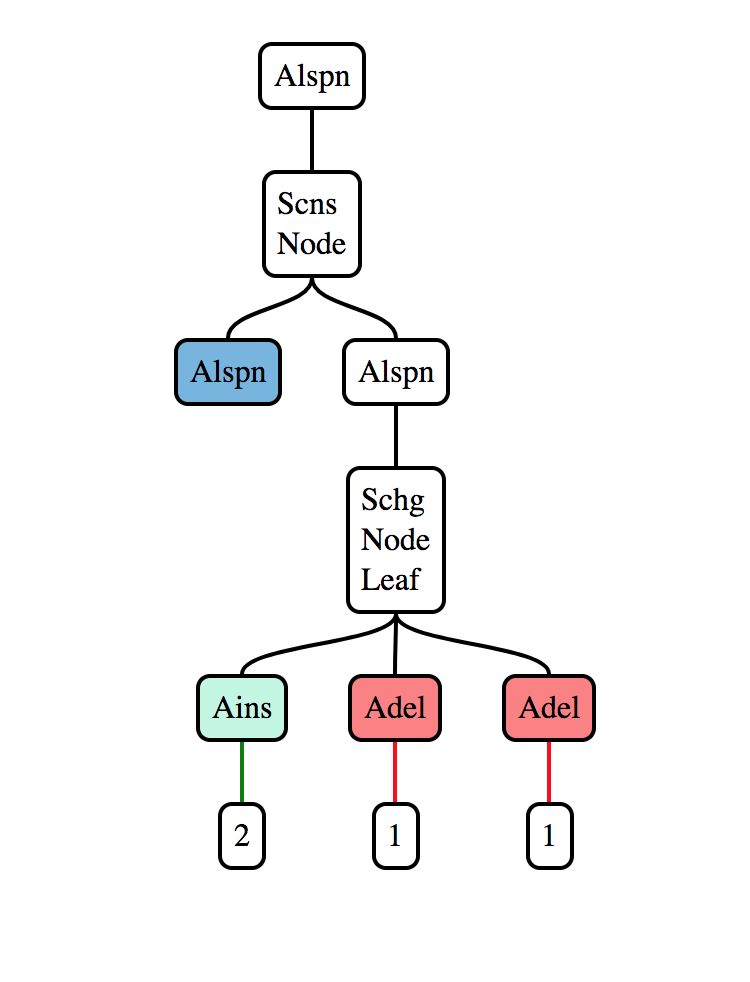
\includegraphics[scale=0.5]{tree.png}
\captionof{figure}{A patch between Binary Trees}
\label{fig:tree}  
\end{minipage}
\\
\\
Recall we are transforming the expression \toClojure{(Node (Leaf 1) (Node (Leaf 1) (Leaf 1)))} to \toClojure{(Node (Leaf 1) (Leaf 2))} -- here we are abusing Clojure notation to represent Binary Trees.

The produced patch correctly shows a copy on the left sub-tree and an \schg on the right one: from a \toClojure{Node} containing two leaves, to a single \toClojure{Leaf} containing a 2. The alignment produced must change the pair of 1s supplied to the source \toClojure{Node} to the single 2 that is the argument to \toClojure{Leaf}. It does so by inserting the 2 and deleting the 1s.

\section{Experimentation}

\subsection{Domain specific improvements}

Before presenting the results we want to introduce a relaxation of the definition of disjointedness. Many of the conflicts appearing in the collected test data share a common pattern. These are conflicts that arise from modifications to configuration files, which in Clojure are often expressed in the language itself via the \toClojure{defproject} macro.
\\
For example:

\begin{minted}{clj}
(defproject project-name "1.2.3"
  :description "The description of the project"
  :dependencies [[dependency-1 "0.0.1"]
     [dependency-2 "1.1.0"]]
  :dev-dependencies [[dev-dependency-1 "1.5.1"]])
\end{minted}

It is very common for these files to give rise to conflicts due to modifications in the required version of the different dependencies by commits which are either merged into, or rebased on top of the development branch. 
\\
\\
We can define two patches to be structurally-disjoint if they only differ on non-recursive atoms. Given a pair of structurally disjoint patches we can employ some domain specific merging strategies which may automate or drastically reduce the user effort required to perform the merge. In a case like the one described above, most of the conflicts are resolved by picking the highest version number every time there is a conflict consisting of a choice between two strings encoding version numbers. Nowadays, most projects adhere to SEMVER \cite{semver} which defines a standard total-ordering for strings representing versions which partially encode the semantics of the change. 
\\
This suggests that conflicts arising from structurally-disjoint patches can often be automatically resolved via some user-defined partial ordering between the atoms of the language. For the case of SEMVER specifically, we could imagine encoding different specific resolution strategies; e.g. we could decide to automatically resolve conflicts between PATCH or MINOR version changes and still notify the user when there is a conflict on a MAJOR version change.
\\
\\
There is another relaxation of the disjointedness predicate which we may consider. The current definition of disjointedness imposes that every patch $p$ -- that is different from the trivial patch \scp -- is not disjoint from itself. We can attempt to relax the definition from disjointedness to compatibility: two compatible patches may modify the same elements, as long as they do so in the same way. It is easy to see that every patch is compatible with itself.
\\
Because of the current practices in how branches and the development process is managed, it is not so rare that we may need to merge a pair of patches which both contain the same changes. These common changes can come from cherry-picking another commit, rebasing, merging or any similar operation between branches of the same repository. Compatible patches can still not be applied in commuting order with the same result unless we relax the definition of application as well. However, it is easy to see that given two patches from the same source, and a proof that they are compatible, we can produce a single patch which encompasses the same changes and is independent of the order in which the two patches are supplied to the function. To put it another way: two patches are compatible if we can combine the into one without throwing away any information and the function that combines them is commutative in its arguments.
Clearly disjointedness implies compatibility by picking the merging function to be the application we defined earlier.

\pdfcomment[icon=Note,color=blue]{This can be made more precise: "without throwing away any information" can be explained better either with commuting diagrams or order (cost) between patches. Last sentence may be confusing as it implies some abuse of notation (application does not produce patches) }

\subsection{Results}
In order to test the framework in a real world context we need to find some suitable data. To acquire this we explored all the Clojure repositories on Github and extracted the ones with the best combination of stars and collaborators. A high number of collaborators will possibly imply a higher chance for conflicts in the source tree, the high number of stars is a good indicator of the quality of the Clojure code and hopefully provides a selection of repositories from different domains.
\\
What we need is a way to identify merge points in a projects history and measure how \diffthree performed in those merges; in essence, we want to find all merge points and record if the merge was performed automatically or a conflict had to be manually resolved.
\\
We wrote some scripts to mine the data from Github and to walk through the source trees mining conflict points that can be used to test the framework. 
\\
Merge commits are identified by the simple fact of being commits that have more than one parent, we will restrict our attention to the case of two parents. This is the most common and sensible case for our scenario, as most teams will develop features on different branches and eventually merge each branch into master. 
This process will generate a merge commit with exactly two parents: one of which is the master branch and the other is the feature branch.
\\
For each of these commits we reproduced the process of performing the merge within branches and extracted any Clojure files that were marked as conflicts from this merge.
\\
For each of these files we want to extract three different versions of it. The original version \mintinline{bash}{O.clj} represents the snapshot of the file at the moment the branches initially diverged. It is the last version the two branches agreed on. We also want to extract the versions \mintinline{bash}{A.clj} and \mintinline{bash}{B.clj}, which capture the current state of the file on each of the two branches.
\\
From this process we obtained 135 folders -- each containing the three different snapshots of the conflicting file. These files have been shrunk with a pre-processing that relies on \diffthree to remove all top level expressions that are are not involved in a conflict in any way.
\\
Each test consists in generating the pair of patches $(OA,OB)$ and checking if they are disjoint. 
The patch $OA$ is the best patch generated between \mintinline{bash}{O.clj} and \mintinline{bash}{A.clj} according to the cost function, and $OB$ is generated in the same way but with \mintinline{bash}{B.clj} as destination.
\\
\\
Conflicts were mined from the following repositories
 \begin{itemize}
    \item clj-http
    \item incanter
    \item lein-figwheel
    \item leiningen
    \item riemann
    \item ring
 \end{itemize}

Out of 135 conflicts, 18 timed out either while constructing the $OA$ or the $OB$ patch; the rest are reported in the following table, showing results of running the tests for disjointedness and compatibility, both in the full and the structurally-respecting variations. 
\\
\begin{center}
 \begin{tabular} { ||c|c|c|c|| }
   \hline Predicate & True & False  \\
   \hline
   \hline Disjoint & 32 & 84 \\
   \hline Structurally-Disjoint & 88 & 28 \\
   \hline Compatible & 42 & 74 \\
   \hline Structurally-Compatible & 97 & 19 \\
   \hline
 \end{tabular}
\end{center}

The relatively small size of test data, especially when compared to the impressive amount of research that has gone in a renowned algorithm as \emph{diff3}, suggests caution in interpreting these results. \\
Having said this, it is certainly encouraging to observe that, given this specific set of conflicts, we perform approximately 20\% better than \diffthree in producing patches that can be safely and automatically merged. We can also see that these numbers drastically increase if we are willing to relax the notion of disjointedness we are investigating. This points to the fact that another strong advantage of this approach -- alongside improving the number of patches which can be automatically merged -- is in the quality of the conflicts that can be produced. Given more accurate information about what is changing between two files enables us to employ stronger conflict resolution rules, which would have been cumbersome, or almost impossible, to express given the "opaque" representation of conflicts from \diffthree
\section{Conclusion}

\subsection{Related Work}\label{rel-work}
In this thesis we focus on converting the theoretical approach presented in \cite{type-directed-diff} into a practical implementation that can be tested against real-world data. Previous attempts to tackle this problems with similar approaches had, nonetheless, some key differences. 
The Untyped approach has been extensively studied: with authors focusing both on the linear \cite{diff, bergroth} and the tree \cite{Akutsu, klein,demanie, billie, autexier, chawalthe} variation. 
\\
In recent years other authors explored the typed approach \cite{Vassena, Lempsink} in a generic setting. However they restricted their attention to the linear variation, by considering a flattening of the tree consisting in a pre-order traversal. The downside is that this flattening makes it harder to guarantee that the transformation encoded in a patch is structurally preserving and thus correct.
\\
Several pieces of related work exist in the literature: from VCS systems built on strong theoretical foundations like Darcs and Pijul, respectively based on work by Roundy \cite{darcs} and Mimram \cite{cat-of-patches}. In our experimentation we have used Git to extract the information required for a merge (e.g. picking the common ancestor between two files). It is interesting to note how O'Connor \cite{git-inconsistent} and other authors point out how the strategy adopted by Git in identifying and picking merge points, is inherently inconsistent and can lead to some surprising outcomes compared to other Version Control Systems.
\\
Remarkably there is a formalization of the theory of patches through the lens of Homotopy Type Theory, which gained a lot of popularity in recent years and offers a new and interesting view on type theory. This has been explored by Licata et al. \cite{HPT} with the key idea of modeling patches as paths in a suitable topological space. 
\\
Finally, Swierstra et al. \cite{semantics-VC} showed how separation logic and Hoare calculus can be used to reason about patches, in particular in terms of characterizing the relationship between patches and defining safe ways in which they can be combined.

\subsection{Future Work}\label{fut-work}

The goal of this work was to explore the performance of the typed, tree-structured diff between datatypes. The result we managed to obtain are surely encouraging, but are still too sparse and specific when confronted with one of the venerable Unix tools as \diff.
\\
Strategies for automatic or semi-automatic conflict resolution where just hinted to in this thesis, exploring them in full generality is probably one of the most important and substantial next steps that can be taken. The definition of application should be modified to convey more information, namely the reason why a certain application failed. 
As mentioned in the previous section regarding SEMVER, we could imagine that some classes of conflicts could be automatically resolved with a custom set of directives specified by end users. Identifying the key use-cases, designing and integrating a framework which allows these custom user-supplied rules is definitely a non-trivial, but possibly very fruitful task.
\\
Finally one of the remaining pieces to fill the puzzle is to explore the level of generality that can be achieved with this approach; while the algorithm is presented generically, the implementation is concretely tied to a specific language: both for convenience of presentation and efficiency. Regardless, for each language, we still need a custom parser to obtain the abstract representation we operate on, which hinders our claim to generality. Of course we can always use a generic strategy to parse a language for which we don't have a more specific parser; in particular one of these generic parsers could be the parser that consumes all characters until a newline. We can imagine that, presented in this context, the original \diff can be collocated at the left end of a scale; by moving to the right we add structural information, which enables us to characterize transformations, and produce more accurate patches. The cost we pay for this is some loss of generality and the added computational complexity. Thus, the final question is ultimately about investigating this balance, the trade-off between adding information and complexity and the (possibly several) "sweet spots" that can be identified in this spectrum.

%Questions
%
% - can we do it globally?
%         How do we pair up nodes?
% - can we do it only on branch?
%         Detect situation before askOracle, if ever true mark some 
%         internal state as deopt and ignore copy information from diff3
% - how many cases can this happen in
%          All nodes that have a pair of subtrees? What about Seq -> Cons



\begin{thebibliography}{30}  
\bibitem{hasochism}
  Lindley, Sam, and Conor McBride. "Hasochism: the pleasure and pain of dependently typed Haskell programming." ACM SIGPLAN Notices 48.12 (2014): 81-92.

\bibitem{singletons} Eisenberg, Richard A., and Stephanie Weirich. "Dependently typed programming with singletons." ACM SIGPLAN Notices 47.12 (2013): 117-130.
  
\bibitem{datakinds} Yorgey, Brent A., et al. "Giving Haskell a promotion." Proceedings of the 8th ACM SIGPLAN workshop on Types in language design and implementation. ACM, 2012.
  
 \bibitem{structure-aware-VC}
   Miraldo, Victor Cacciari, and Wouter Swierstra. "Structure-aware version control: A generic approach using Agda." (2017).

\bibitem{semantics-VC} 
   Swierstra, Wouter, and Andres Loh. "The semantics of version control." Proceedings of the 2014 ACM International Symposium on New Ideas, New Paradigms, and Reflections on Programming and Software. ACM, 2014.

\bibitem{type-directed-diff}
  Miraldo, Victor Cacciari, Pierre-Évariste Dagand, and Wouter Swierstra. "Type-directed diffing of structured data." Proceedings of the 2nd ACM SIGPLAN International Workshop on Type-Driven Development. ACM, 2017.
  
\bibitem{true-sop}
  de Vries, Edsko, and Andres Löh. "True sums of products." Proceedings of the 10th ACM SIGPLAN workshop on Generic programming. ACM, 2014.
  
\bibitem{clojure}
Hickey, Rich. "The clojure programming language." Proceedings of the 2008 symposium on Dynamic languages. ACM, 2008.

\bibitem{dependent-haskell} Eisenberg, Richard A. "Dependent types in Haskell: Theory and practice." arXiv preprint arXiv:1610.07978 (2016). APA	

\bibitem{zippers} Huet, Gérard. "The zipper." Journal of functional programming 7.5 (1997): 549-554.

\bibitem{treant} http://fperucic.github.io/treant-js/

\bibitem{semver} https://semver.org/

\bibitem{darcs} Roundy, David. "Darcs: distributed version management in haskell." Proceedings of the 2005 ACM SIGPLAN workshop on Haskell. ACM, 2005.

\bibitem{HPT} Angiuli, Carlo, et al. "Homotopical patch theory." ACM SIGPLAN Notices. Vol. 49. No. 9. ACM, 2014.

\bibitem{Akutsu} Akutsu, Tatsuya, Daiji Fukagawa, and Atsuhiro Takasu. "Approximating tree edit distance through string edit distance." Algorithmica 57.2 (2010): 325-348.

\bibitem{diff} Hunt, James Wayne, and M. D. MacIlroy. An algorithm for differential file comparison. Murray Hill: Bell Laboratories, 1976.

\bibitem{bergroth} Bergroth, Lasse, Harri Hakonen, and Timo Raita. "A survey of longest common subsequence algorithms." String Processing and Information Retrieval, 2000. SPIRE 2000. Proceedings. Seventh International Symposium on. IEEE, 2000.

\bibitem{klein} Klein, Philip N. "Computing the edit-distance between unrooted ordered trees." ESA. Vol. 98. 1998.

\bibitem{demanie} Demaine, Erik D., et al. "An optimal decomposition algorithm for tree edit distance." ACM Transactions on Algorithms (TALG) 6.1 (2009): 2.

\bibitem{billie} Bille, Philip. "A survey on tree edit distance and related problems." Theoretical computer science 337.1 (2005): 217-239.

\bibitem{autexier} Autexier, Serge. "Similarity-Based Diff, Three-Way Diff and Merge." International Journal of Software and Informatics 9.2 (2015).

\bibitem{chawalthe} Chawathe, Sudarshan S., and Hector Garcia-Molina. "Meaningful change detection in structured data." ACM SIGMOD Record. Vol. 26. No. 2. ACM, 1997.

\bibitem{Lempsink} Lempsink, Eelco, Sean Leather, and Andres Löh. "Type-safe diff for families of datatypes." Proceedings of the 2009 ACM SIGPLAN workshop on Generic programming. ACM, 2009.

\bibitem{Vassena} Vassena, Marco. "Generic Diff3 for algebraic datatypes." Proceedings of the 1st International Workshop on Type-Driven Development. ACM, 2016.

\bibitem{cat-of-patches} Mimram, Samuel, and Cinzia Di Giusto. "A categorical theory of patches." Electronic notes in theoretical computer science 298 (2013): 283-307.

\bibitem{git-inconsistent} http://r6.ca/blog/20110416T204742Z.html
\end{thebibliography}
\end{document}  
